\documentclass[12pt,a4paper]{article}

% Компиляция: pdflatex main.tex (два раза).
% Оформление титульного листа воспроизводит образец отчёта 3.4.5.
\usepackage[T2A]{fontenc}
\usepackage[utf8]{inputenc}
\usepackage[russian]{babel}
\usepackage{amsmath,amssymb}
\usepackage{graphicx}
\usepackage{float}
\usepackage{booktabs}
\usepackage{array}
\usepackage{tikz}
\usepackage[left=2.5cm,right=1cm,top=2cm,bottom=2cm]{geometry}

\setlength{\parindent}{1.25cm}
\setlength{\parskip}{0pt}
\renewcommand{\figurename}{Рис.}
\renewcommand{\tablename}{Таблица}

% Все рисунки расположены непосредственно после соответствующего абзаца.
% Все изображения сохраняйте в папке figures рядом с main.tex.
% Схема: figures/scheme.png; графики: calibration.png, hall.png, slope.png.
% Пока графика нет, выводится текстовое примечание.
% Не изменяйте "[H]" — это предотвращает перенос рисунков по документу.
\newcommand{\emptycell}{\rule{0.8cm}{0pt}}

\begin{document}

% --------------------------------------------------
% ТИТУЛЬНЫЙ ЛИСТ — композиция, типографика, положение
% элементов сохранены по примеру lab 3.4.5.
% --------------------------------------------------
\begin{titlepage}
\thispagestyle{empty}
\begin{tikzpicture}[remember picture,overlay]
  \coordinate (NW) at (current page.north west);
  \node[anchor=center,inner sep=0pt] at ([xshift=319.8pt,yshift=-66.8pt]NW)
    {\Large Московский Физико-Технический Институт};

  \node[anchor=center,inner sep=0pt] at ([xshift=319.8pt,yshift=-202.5pt]NW)
    {\Large Лабораторная работа №3.3.4};

  \draw[line width=0.4pt] ([xshift=84.68pt,yshift=-235.12pt]NW) --
                           ([xshift=549.94pt,yshift=-235.12pt]NW);
  \node[anchor=center,inner sep=0pt] at ([xshift=319.8pt,yshift=-270.1pt]NW)
    {\huge\bfseries Эффект Холла};
  \node[anchor=center,inner sep=0pt] at ([xshift=319.8pt,yshift=-303.2pt]NW)
    {\huge\bfseries в полупроводниках};
  \draw[line width=0.4pt] ([xshift=84.68pt,yshift=-329.77pt]NW) --
                           ([xshift=549.94pt,yshift=-329.77pt]NW);

  \node[anchor=north west,inner sep=0pt,align=left,font=\large]
    at ([xshift=357.4pt,yshift=-515.3pt]NW) {
      Выполнил:\\[-1.1pt]
      Студент 2 курса ФАКТ\\[-1.1pt]
      Группа Б03-502\\[-1.1pt]
      Подмосковнов Лев
    };

  \node[anchor=center,inner sep=0pt] at ([xshift=319.8pt,yshift=-768pt]NW)
    {\large Долгопрудный};
  \node[anchor=center,inner sep=0pt] at ([xshift=319.8pt,yshift=-784pt]NW)
    {\large 2026};
\end{tikzpicture}
\null
\end{titlepage}

\section*{Цель работы}
Измерение подвижности и концентрации носителей заряда в полупроводниках.

\section*{Используемые приборы и материалы}
В работе используются:
\begin{itemize}
  \item электромагнит с регулируемым источником питания;
  \item вольтметр, амперметр и миллиамперметр;
  \item милливеберметр или миллитесламетр;
  \item источник питания образца (1,5 В);
  \item образец легированного германия.
\end{itemize}

\section{Теоретическое введение}

\subsection{Эффект Холла}
При протекании тока $I$ через полупроводниковую пластинку,
помещённую в магнитное поле $\mathbf B$, перпендикулярное её
плоскости, на носители заряда действует магнитная составляющая
силы Лоренца. Разделение зарядов создаёт поперечное электрическое
поле и разность потенциалов $U_{\perp}$ между краями образца.

Для образца толщиной $h$ в однозонном приближении с одним
преобладающим типом носителей справедливо соотношение
\begin{equation}
    U_{\perp}=R_H\frac{BI}{h},\qquad R_H=\frac{1}{nq},
    \label{eq:hall}
\end{equation}
где $R_H$ --- постоянная Холла, $n$ --- концентрация носителей,
$q$ --- их заряд с учётом знака. Знак $R_H$ определяется типом
основных носителей заряда.

\subsection{Выделение ЭДС Холла}
Из-за несовершенства расположения измерительных контактов
напряжение $U_{34}$ содержит также омическую составляющую $U_0$.
Её определяют при отсутствии магнитного поля при том же токе
$I$ через образец. Тогда
\begin{equation}
    U_{\perp}=U_{34}-U_0.
    \label{eq:correction}
\end{equation}
При измерениях для противоположных направлений магнитного поля
возможно также использовать полуразность:
\begin{equation}
    U_{\perp}=\frac{U_{34}^{(+)}-U_{34}^{(-)}}{2}.
\end{equation}

\subsection{Определение параметров полупроводника}
При постоянном токе $I$ зависимость $U_{\perp}(B)$ должна быть
линейной. Её угловой коэффициент и зависимость этого коэффициента
от тока выражаются как
\begin{equation}
    k=\frac{dU_{\perp}}{dB}=\frac{R_H I}{h},
    \qquad
    R_H=h\frac{dk}{dI}.
    \label{eq:slopes}
\end{equation}
Концентрация носителей заряда:
\begin{equation}
    n=\frac{1}{e\lvert R_H\rvert},
    \label{eq:concentration}
\end{equation}
где $e$ --- модуль элементарного заряда.

По продольному падению напряжения $U_{35}$ на участке длиной $l$
при ширине образца $a$ определяется удельное сопротивление:
\begin{equation}
    \rho_0=\frac{U_{35}}{I}\frac{ah}{l},\qquad
    \sigma_0=\frac{1}{\rho_0},\qquad
    \mu=\lvert R_H\rvert\sigma_0.
    \label{eq:transport}
\end{equation}
Подвижность $\mu$ в окончательном ответе выражается в
$\text{см}^2/(\text{В}\cdot\text{с})$.

\subsection{Экспериментальная установка}
В зазоре электромагнита расположен образец легированного
германия. Ток через образец регулируется реостатом и измеряется
миллиамперметром. Напряжение между холловскими контактами 3 и 4
измеряется вольтметром. Индукция поля определяется по градуировке
электромагнита.

\begin{figure}[H]
    \centering
    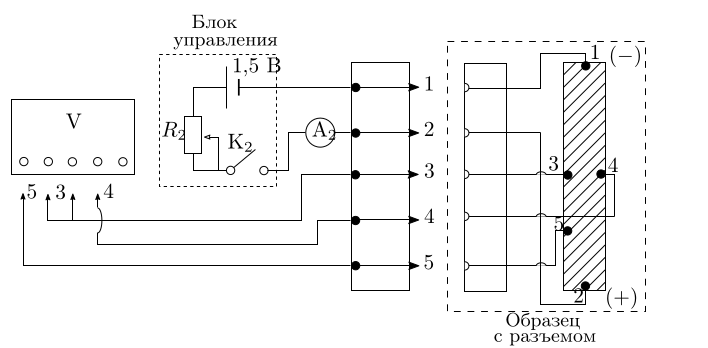
\includegraphics[width=0.85\textwidth,keepaspectratio]{figures/scheme.png}
    \caption{Схема установки для исследования эффекта Холла в полупроводниках}
    \label{fig:setup}
\end{figure}

\newpage

\section{Ход работы и результаты измерений}

\subsection{Параметры образца и характеристики приборов}
В таблице~\ref{tab:params} приведены известные геометрические
параметры исследуемого образца.

\begin{table}[H]
\centering
\caption{Геометрические параметры исследуемого образца}
\label{tab:params}
\begin{tabular}{@{}lll@{}}
\toprule
Величина & Обозначение & Значение \\
\midrule
Расстояние между контактами 3 и 5 & $l$ & $3{,}0$ мм \\
Ширина образца & $a$ & $2{,}2$ мм \\
Толщина образца & $h$ & $2{,}5$ мм \\
\bottomrule
\end{tabular}
\end{table}


\subsection{Градуировка электромагнита}
Магнитная индукция $B$ измерялась непосредственно в миллитеслах при
изменении тока $I_M$ в обмотке электромагнита. Все записанные
экспериментальные значения приведены в таблице~\ref{tab:calib}.
При обработке результатов поле в промежуточных точках находилось
линейной интерполяцией соседних измерений.

\begin{table}[H]
\centering
\caption{Градуировка электромагнита}
\label{tab:calib}
\begin{tabular}{@{}ccc@{}}
\toprule
$I_M$, А & $B$, мТл & $B$, Тл \\
\midrule
0{,}08 & 94 & 0{,}094 \\
0{,}19 & 219 & 0{,}219 \\
0{,}39 & 423 & 0{,}423 \\
0{,}59 & 614 & 0{,}614 \\
0{,}79 & 771 & 0{,}771 \\
1{,}00 & 895 & 0{,}895 \\
1{,}20 & 970 & 0{,}970 \\
1{,}39 & 1017 & 1{,}017 \\
1{,}68 & 1056 & 1{,}056 \\
\bottomrule
\end{tabular}
\end{table}

\subsection{Измерение поперечного напряжения}
Для пяти токов $I$ через образец измерялись напряжение $U_0$ в
отсутствие магнитного поля и напряжение $U_{34}$ при различном токе
электромагнита $I_M$. В исходной тетради напряжение записано в
\textbf{мкВ}; пересчёт в мВ не производился.

\begin{table}[H]
\centering
\caption{Смещения при нулевом магнитном поле}
\label{tab:u0}
\begin{tabular}{@{}cc@{}}
\toprule
$I$, мА & $U_0$, мкВ \\
\midrule
0{,}2 & -3 \\
0{,}4 & -11 \\
0{,}6 & -19 \\
0{,}8 & -26 \\
1{,}0 & -34 \\
\bottomrule
\end{tabular}
\end{table}

\subsubsection*{Ток через образец $I=0{,}2$ мА}
\begin{table}[H]
\centering
\caption{Результаты измерений при $I=0{,}2$ мА}
\label{tab:hall02}
\begin{tabular}{@{}cccc@{}}
\toprule
$I_M$, А & $B$, Тл & $U_{34}$, мкВ & $U_\perp$, мкВ \\
\midrule
0{,}21 & 0{,}239 & -12 & -9 \\
0{,}40 & 0{,}433 & -20 & -17 \\
0{,}59 & 0{,}614 & -27 & -24 \\
0{,}80 & 0{,}777 & -33 & -30 \\
1{,}01 & 0{,}899 & -38 & -35 \\
1{,}20 & 0{,}970 & -41 & -38 \\
1{,}40 & 1{,}018 & -44 & -41 \\
1{,}58 & 1{,}043 & -45 & -42 \\
\bottomrule
\end{tabular}
\end{table}
\subsubsection*{Ток через образец $I=0{,}4$ мА}
\begin{table}[H]
\centering
\caption{Результаты измерений при $I=0{,}4$ мА}
\label{tab:hall04}
\begin{tabular}{@{}cccc@{}}
\toprule
$I_M$, А & $B$, Тл & $U_{34}$, мкВ & $U_\perp$, мкВ \\
\midrule
0{,}21 & 0{,}239 & -27 & -16 \\
0{,}41 & 0{,}442 & -42 & -31 \\
0{,}60 & 0{,}622 & -57 & -46 \\
0{,}80 & 0{,}777 & -69 & -58 \\
1{,}01 & 0{,}899 & -79 & -68 \\
1{,}19 & 0{,}966 & -85 & -74 \\
1{,}40 & 1{,}018 & -90 & -79 \\
1{,}58 & 1{,}043 & -94 & -83 \\
\bottomrule
\end{tabular}
\end{table}
\subsubsection*{Ток через образец $I=0{,}6$ мА}
При $I_M=0{,}20$ А измерено $U_{34}=-42$ мкВ. При $U_0=-19$ мкВ получаем $U_{\perp}=-23$ мкВ; точка учтена при аппроксимации.

\begin{table}[H]
\centering
\caption{Результаты измерений при $I=0{,}6$ мА}
\label{tab:hall06}
\begin{tabular}{@{}cccc@{}}
\toprule
$I_M$, А & $B$, Тл & $U_{34}$, мкВ & $U_\perp$, мкВ \\
\midrule
0{,}20 & 0{,}229 & -42 & -23 \\
0{,}41 & 0{,}442 & -65 & -46 \\
0{,}61 & 0{,}630 & -87 & -68 \\
0{,}81 & 0{,}783 & -105 & -86 \\
1{,}00 & 0{,}895 & -119 & -100 \\
1{,}21 & 0{,}972 & -130 & -111 \\
1{,}41 & 1{,}020 & -137 & -118 \\
1{,}57 & 1{,}041 & -142 & -123 \\
\bottomrule
\end{tabular}
\end{table}
\subsubsection*{Ток через образец $I=0{,}8$ мА}
\begin{table}[H]
\centering
\caption{Результаты измерений при $I=0{,}8$ мА}
\label{tab:hall08}
\begin{tabular}{@{}cccc@{}}
\toprule
$I_M$, А & $B$, Тл & $U_{34}$, мкВ & $U_\perp$, мкВ \\
\midrule
0{,}20 & 0{,}229 & -60 & -34 \\
0{,}41 & 0{,}442 & -89 & -63 \\
0{,}60 & 0{,}622 & -115 & -89 \\
0{,}82 & 0{,}789 & -143 & -117 \\
1{,}00 & 0{,}895 & -160 & -134 \\
1{,}20 & 0{,}970 & -179 & -153 \\
1{,}40 & 1{,}018 & -184 & -158 \\
1{,}57 & 1{,}041 & -191 & -165 \\
\bottomrule
\end{tabular}
\end{table}
\subsubsection*{Ток через образец $I=1{,}0$ мА}
\begin{table}[H]
\centering
\caption{Результаты измерений при $I=1{,}0$ мА}
\label{tab:hall10}
\begin{tabular}{@{}cccc@{}}
\toprule
$I_M$, А & $B$, Тл & $U_{34}$, мкВ & $U_\perp$, мкВ \\
\midrule
0{,}21 & 0{,}239 & -74 & -40 \\
0{,}40 & 0{,}433 & -110 & -76 \\
0{,}60 & 0{,}622 & -145 & -111 \\
0{,}82 & 0{,}789 & -179 & -145 \\
1{,}01 & 0{,}899 & -201 & -167 \\
1{,}20 & 0{,}970 & -219 & -185 \\
1{,}40 & 1{,}018 & -251 & -217 \\
1{,}57 & 1{,}041 & -240 & -206 \\
\bottomrule
\end{tabular}
\end{table}

\subsection{Измерения при обратном направлении магнитного поля}
При токе через образец $I=1{,}0$ мА направление магнитного поля
изменяли на противоположное. Показания вольтметра для обратного
направления поля приведены отдельно, без искусственного
приравнивания близких, но не одинаковых токов $I_M$.

\begin{table}[H]
\centering
\caption{Измерения с обратной полярностью поля при $I=1{,}0$ мА}
\label{tab:reverse}
\begin{tabular}{@{}ccc@{}}
\toprule
$I_M$, А & $|B|$, Тл & $U_{34}^{(-)}$, мкВ \\
\midrule
0{,}21 & 0{,}239 & 5 \\
0{,}41 & 0{,}442 & 45 \\
0{,}61 & 0{,}630 & 74 \\
0{,}81 & 0{,}783 & 110 \\
1{,}01 & 0{,}899 & 155 \\
1{,}20 & 0{,}970 & 150 \\
1{,}40 & 1{,}018 & 164 \\
1{,}56 & 1{,}040 & 172 \\
\bottomrule
\end{tabular}
\end{table}

\begin{samepage}
По направлениям тока через образец и магнитного поля, а также
по знаку измеренной ЭДС Холла экспериментально определён знак
основных носителей заряда:
\[
    q=-e.
\]
Следовательно, носителями заряда являются электроны, а образец
имеет электронный тип проводимости ($n$-тип).
\end{samepage}

\subsection{Измерение продольного падения напряжения}
При отсутствии магнитного поля и при максимальном токе через
образец $I=1{,}0$ мА измерено продольное напряжение между
контактами 3 и 5:
\[
    U_{35}=1741\ \text{мкВ}.
\]



\section{Обработка результатов}

\subsection{Градуировочная зависимость $B(I_M)$}
Градуировочная зависимость $B(I_M)$ построена по результатам
измерений, приведённым в таблице~\ref{tab:calib}.
Для определения индукции при промежуточных значениях тока
электромагнита использована линейная интерполяция между
соседними экспериментальными точками.

\begin{figure}[H]
    \centering
    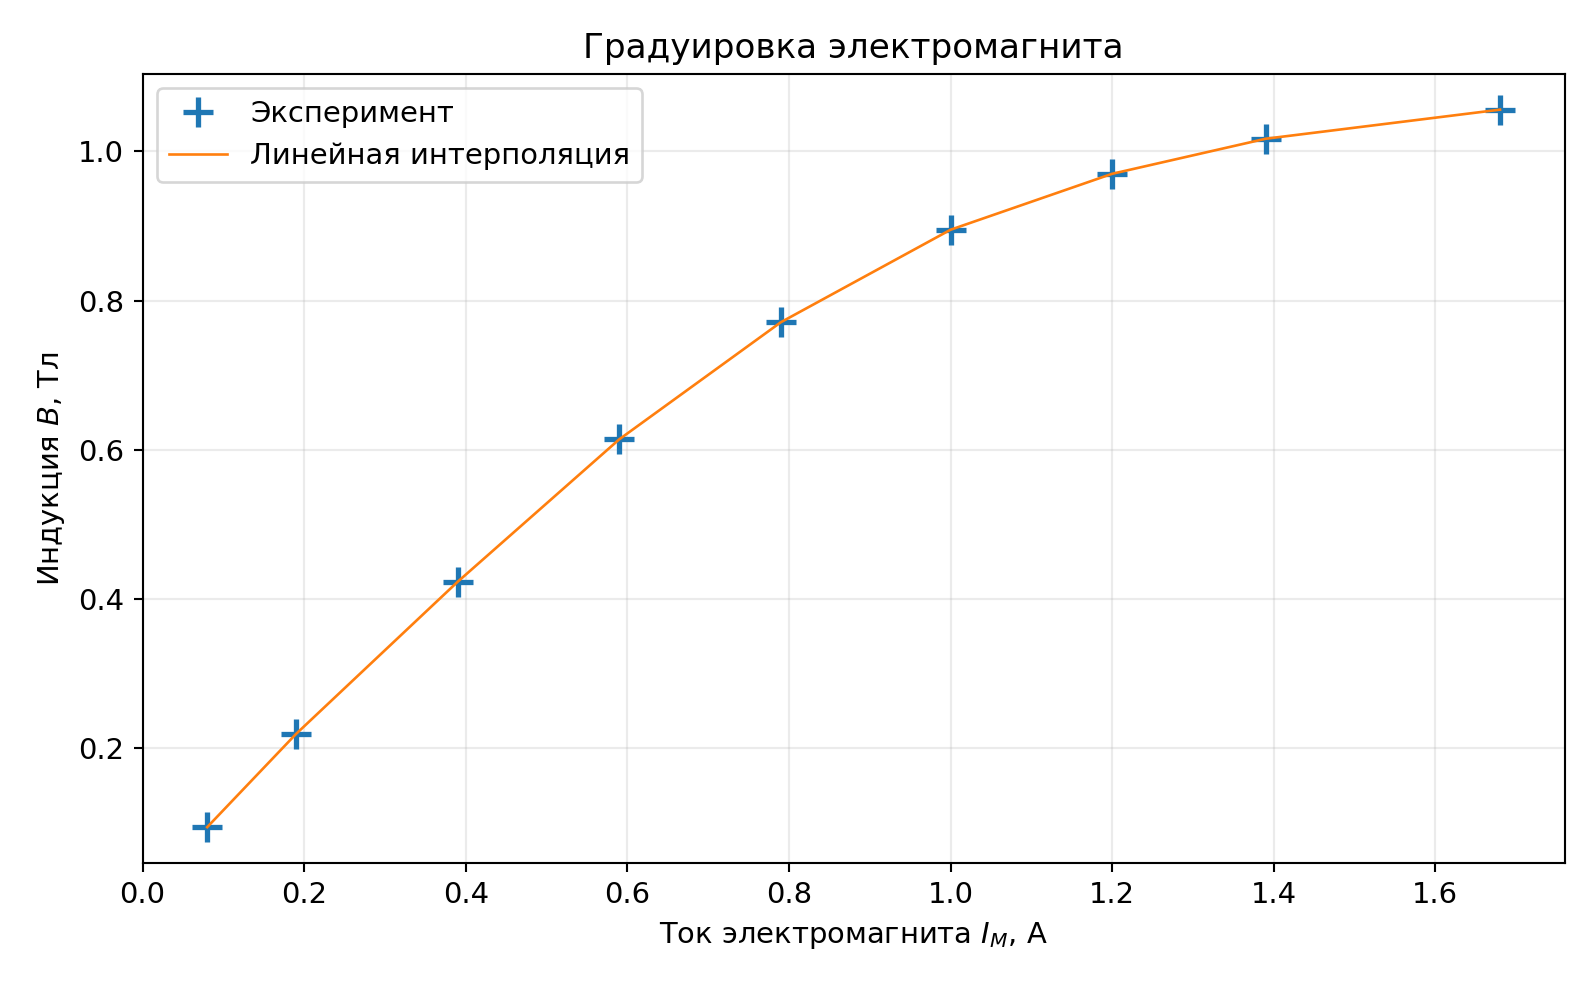
\includegraphics[width=0.85\textwidth,keepaspectratio]{figures/calibration.png}
    \caption{Зависимость магнитной индукции $B$ от силы тока в обмотке электромагнита $I_M$}
    \label{fig:calibration}
\end{figure}

% 0.6 мА: включена точка (0.229 Тл, -23 мкВ), графики и МНК пересчитаны.
\subsection{Семейство зависимостей $U_{\perp}(B)$}
В каждой серии из показаний вольтметра вычиталось соответствующее
смещение $U_0$. На графике показаны экспериментальные точки и отдельно прямые,
найденные методом наименьших квадратов при свободном члене:
\[
    U_\perp=kB+b.
\]
Все восемь измеренных точек серии $I=0{,}6$ мА включены
в аппроксимацию.

\begin{figure}[H]
    \centering
    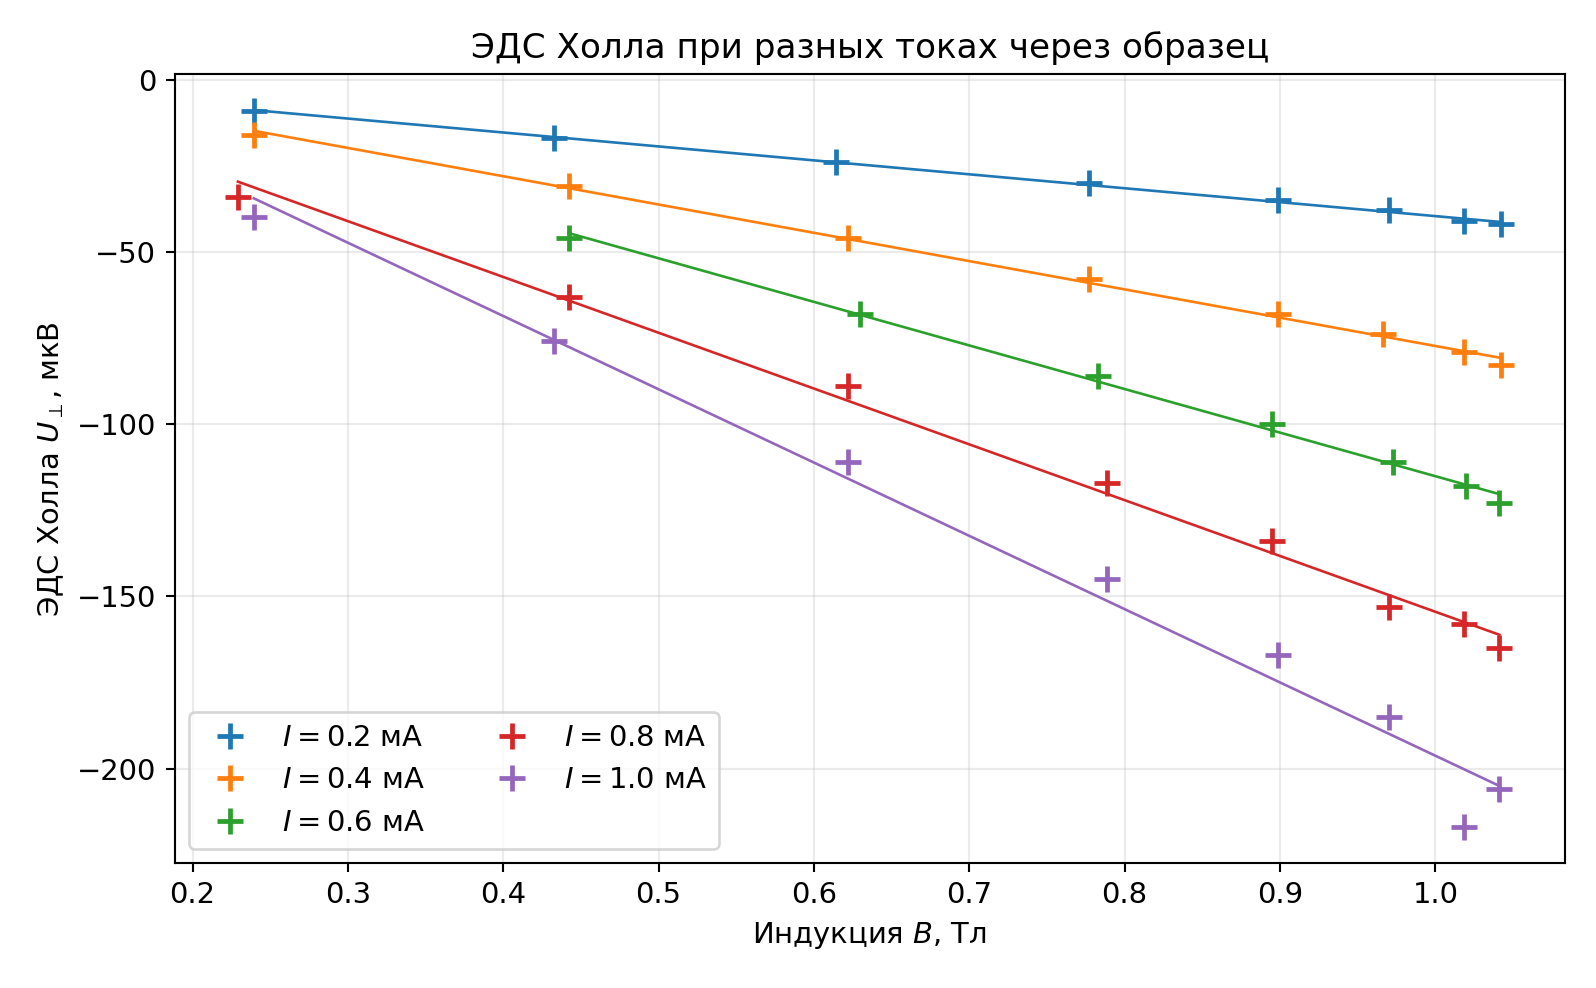
\includegraphics[width=0.85\textwidth,keepaspectratio]{figures/hall.png}
    \caption{Зависимость ЭДС Холла $U_{\perp}$ от магнитной индукции $B$ при различных значениях силы тока через образец $I$}
    \label{fig:hall}
\end{figure}

\begin{table}[H]
\centering
\caption{Параметры линейных аппроксимаций $U_\perp(B)$}
\label{tab:slopes}
\begin{tabular}{@{}cccc@{}}
\toprule
$I$, мА & $k$, мкВ/Тл & $u(k)$, мкВ/Тл & $R^2$ \\
\midrule
0{,}2 & -40{,}5 & 0{,}7 & 0{,}998 \\
0{,}4 & -82{,}1 & 1{,}6 & 0{,}998 \\
0{,}6 & -121{,}9 & 2{,}8 & 0{,}997 \\
0{,}8 & -162{,}0 & 4{,}9 & 0{,}995 \\
1{,}0 & -212{,}7 & 11{,}3 & 0{,}983 \\
\bottomrule
\end{tabular}
\end{table}

Здесь $u(k)$ --- стандартная ошибка углового коэффициента при
аппроксимации МНК.

\subsection{Постоянная Холла и концентрация носителей}
По таблице~\ref{tab:slopes} построена зависимость $k(I)$,
аппроксимированная прямой $k=sI+k_0$. Для вычислений ток $I$
переведён в амперы, а $k$ --- в В/Тл.

\begin{figure}[H]
    \centering
    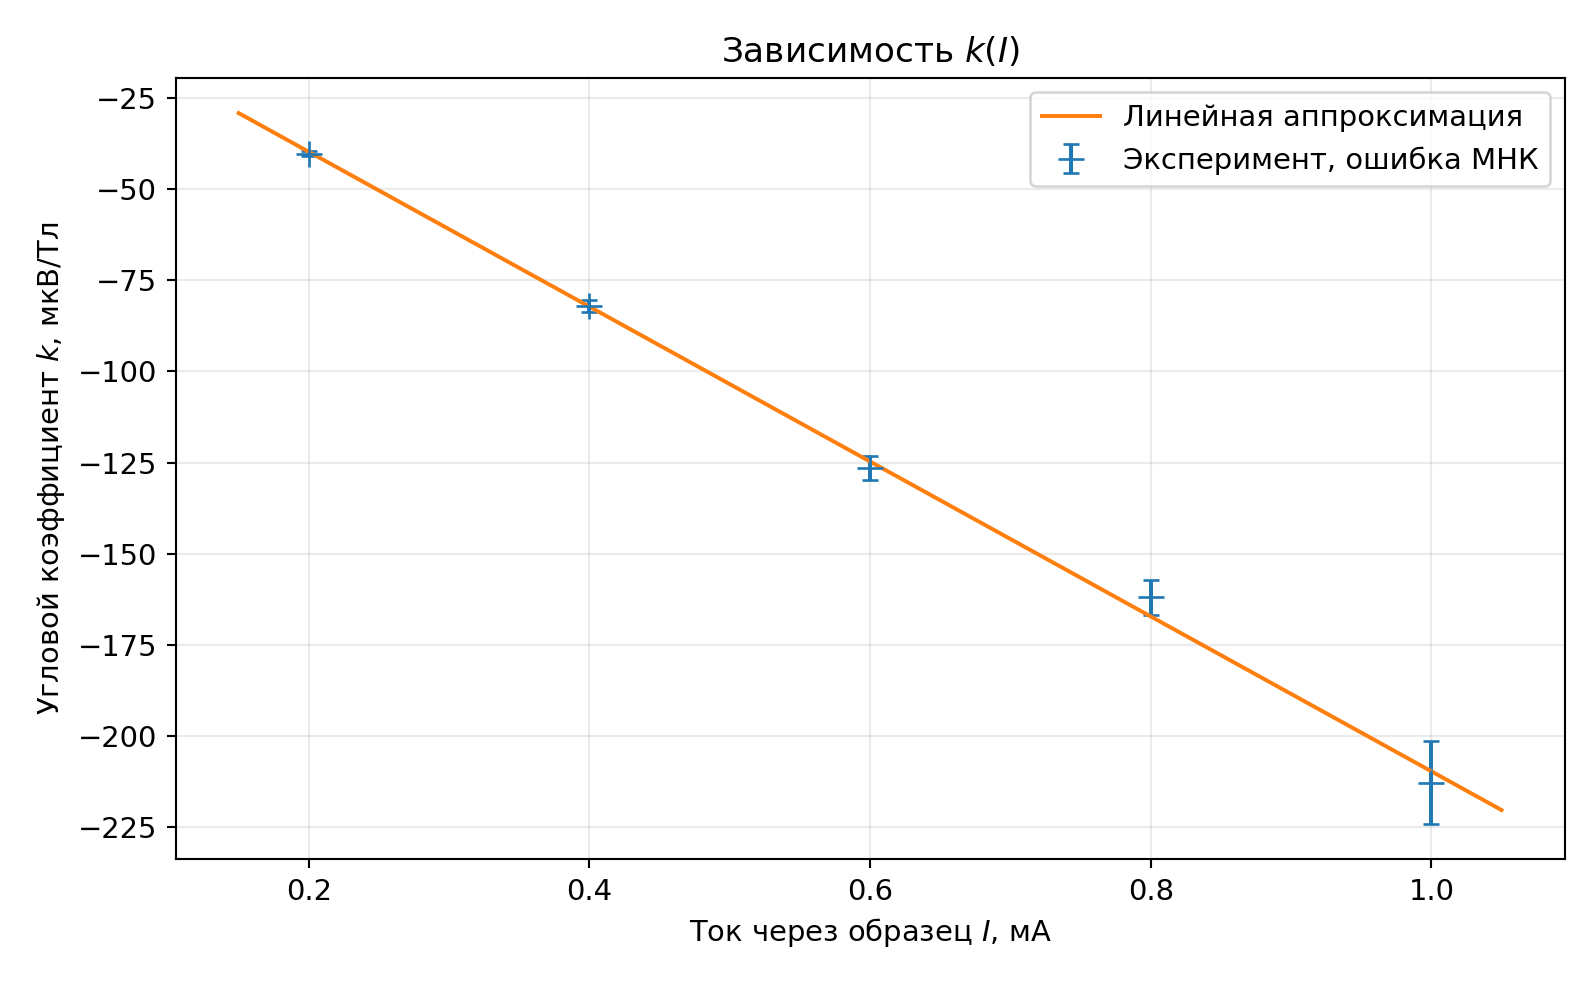
\includegraphics[width=0.85\textwidth,keepaspectratio]{figures/slope.png}
    \caption{Зависимость углового коэффициента $k$ от силы тока через образец $I$}
    \label{fig:slope}
\end{figure}


\begin{align}
 s &= (-0{,}212\pm0{,}006)\ \frac{\text{В}}{\text{Тл}\cdot\text{А}},\\
 R_H &= hs=(-5{,}30\pm0{,}15)\cdot 10^{-4}\ \frac{\text{м}^3}{\text{Кл}},\\
 n &= \frac{1}{e|R_H|}=(1{,}18\pm0{,}03)\cdot10^{22}\ \text{м}^{-3}.
\end{align}

\noindent В скобках приведены только статистические неопределённости,
полученные из линейной регрессии при фиксированной толщине $h$;
погрешности геометрии и приборов сюда не включены.

Отрицательное значение постоянной Холла согласуется с
экспериментально определённым отрицательным зарядом основных
носителей. Таким образом, исследуемый образец имеет электронный
тип проводимости ($n$-тип).

\subsection{Удельное сопротивление, проводимость и подвижность}
При вычислении характеристик образца использованы измеренное
продольное напряжение $U_{35}=1741$ мкВ, ток $I=1{,}0$ мА
и геометрические параметры $a=2{,}2$ мм, $h=2{,}5$ мм,
$l=3{,}0$ мм.


\begin{align}
 \rho_0 &=\frac{U_{35}}{I}\frac{ah}{l}=3{,}19\cdot10^{-3}\ \text{Ом}\cdot\text{м},\\
 \sigma_0 &=\frac{1}{\rho_0}=313\ \frac{\text{См}}{\text{м}},\\
 \mu &=|R_H|\sigma_0=1{,}66\cdot10^{3}\ \frac{\text{см}^2}{\text{В}\cdot\text{с}}.
\end{align}

\subsection{Оценка погрешностей}

Стандартные ошибки угловых коэффициентов $k$ и $s$ были
определены методом наименьших квадратов. Для постоянной Холла
и концентрации носителей заряда ранее получены статистические
погрешности:
\begin{align}
 R_H &=(-5{,}30\pm0{,}15)\cdot10^{-4}\
       \frac{\text{м}^3}{\text{Кл}},\\
 n &=(1{,}18\pm0{,}03)\cdot10^{22}\ \text{м}^{-3}.
\end{align}

Для оценки погрешностей удельного сопротивления,
проводимости и подвижности, поскольку паспортная точность
приборов не указана, условно примем половину единицы
последнего записанного разряда:
\begin{align*}
 \Delta U_{35}&=0{,}5\ \text{мкВ},&
 \Delta I&=0{,}05\ \text{мА},\\
 \Delta a&=0{,}05\ \text{мм},&
 \Delta h&=0{,}05\ \text{мм},&
 \Delta l&=0{,}05\ \text{мм}.
\end{align*}
Это оценки по округлению записанных значений, а не полные
приборные погрешности. Будем считать погрешности исходных
измерений независимыми.

Для удельного сопротивления
\begin{equation}
 \rho_0=\frac{U_{35}ah}{Il}
\end{equation}
относительная погрешность составляет
\begin{equation}
 \frac{\Delta\rho_0}{\rho_0}=
 \sqrt{
 \left(\frac{\Delta U_{35}}{U_{35}}\right)^2+
 \left(\frac{\Delta a}{a}\right)^2+
 \left(\frac{\Delta h}{h}\right)^2+
 \left(\frac{\Delta I}{I}\right)^2+
 \left(\frac{\Delta l}{l}\right)^2
 }
 =0{,}0608.
\end{equation}
Следовательно,
\begin{equation}
 \rho_0=(3{,}19\pm0{,}19)\cdot10^{-3}\
         \text{Ом}\cdot\text{м}.
\end{equation}

Для проводимости $\sigma_0=1/\rho_0$:
\begin{equation}
 \frac{\Delta\sigma_0}{\sigma_0}
 =\frac{\Delta\rho_0}{\rho_0}
 =0{,}0608,
 \qquad
 \sigma_0=(313\pm19)\ \frac{\text{См}}{\text{м}}.
\end{equation}

При оценке погрешности подвижности учтём, что
$R_H=hs$ и $\rho_0=U_{35}ah/(Il)$ содержат
\emph{одну и ту же} измеренную толщину $h$.
Поэтому при вычислении $\mu=|R_H|/\rho_0$
толщина сокращается:
\begin{equation}
 \mu=\frac{|s|Il}{U_{35}a}.
\end{equation}
Тогда, не учитывая толщину дважды, получаем
\begin{equation}
 \frac{\Delta\mu}{\mu}=
 \sqrt{
 \left(\frac{\Delta s}{s}\right)^2+
 \left(\frac{\Delta I}{I}\right)^2+
 \left(\frac{\Delta l}{l}\right)^2+
 \left(\frac{\Delta U_{35}}{U_{35}}\right)^2+
 \left(\frac{\Delta a}{a}\right)^2
 }
 =0{,}0640,
\end{equation}
где $\Delta s=0{,}006\ \text{В}/(\text{Тл}\cdot\text{А})$
--- статистическая неопределённость МНК.
Таким образом,
\begin{equation}
 \mu=(1{,}66\pm0{,}11)\cdot10^3\
       \frac{\text{см}^2}{\text{В}\cdot\text{с}}.
\end{equation}

\begin{table}[H]
\centering
\caption{Полученные характеристики образца с погрешностями}
\label{tab:summary}
\begin{tabular}{@{}lll@{}}
\toprule
Величина & Результат & Единица \\
\midrule
$R_H$ & $(-5{,}30\pm0{,}15)\cdot10^{-4}$ &
м$^3$/Кл (стат.) \\
$n$ & $(1{,}18\pm0{,}03)\cdot10^{22}$ &
м$^{-3}$ (стат.) \\
$\rho_0$ & $(3{,}19\pm0{,}19)\cdot10^{-3}$ & Ом$\cdot$м \\
$\sigma_0$ & $313\pm19$ & См/м \\
$\mu$ & $(1{,}66\pm0{,}11)\cdot10^3$ &
см$^2$/(В$\cdot$с) \\
\bottomrule
\end{tabular}
\end{table}
Полученные для $\rho_0$, $\sigma_0$ и $\mu$ погрешности
предварительные и зависят от принятых выше оценок
точности измерений.

\section*{Вывод}

Был экспериментально определён отрицательный знак основных
носителей заряда, соответствующий электронной проводимости
образца ($n$-тип):
\[
    q=-e.
\]

Была рассчитана постоянная Холла $R_H$:
\[
 R_H=(-5{,}30\pm0{,}15)\cdot10^{-4}\
 \frac{\text{м}^3}{\text{Кл}}.
\]

Была определена концентрация носителей заряда $n$:
\[
 n=(1{,}18\pm0{,}03)\cdot10^{22}\ \text{м}^{-3}.
\]

Было рассчитано удельное сопротивление $\rho_0$:
\[
 \rho_0=(3{,}19\pm0{,}19)\cdot10^{-3}\
 \text{Ом}\cdot\text{м}.
\]

Была вычислена удельная электрическая проводимость $\sigma_0$:
\[
 \sigma_0=(313\pm19)\ \frac{\text{См}}{\text{м}}.
\]

Была определена подвижность носителей заряда $\mu$:
\[
 \mu=(1{,}66\pm0{,}11)\cdot10^3\
 \frac{\text{см}^2}{\text{В}\cdot\text{с}}.
\]

\end{document}
